\documentclass{standalone}
\usepackage{tikz,pgfplots}
\pgfplotsset{compat=1.16}
\usetikzlibrary{arrows,positioning}
\usetikzlibrary{plotmarks}
\usetikzlibrary{backgrounds,arrows.meta,external,babel,math,patterns,patterns.meta,calc,decorations.pathmorphing,decorations.markings, decorations.pathreplacing,shapes,fillbetween}
\newcommand{\AxisRotator}[1][rotate=0]{%
	\tikz [x=0.25cm,y=0.60cm,line width=.2ex,-stealth,#1] \draw (0,0) arc (-150:150:1 and 1);%
}
\begin{document}
    \begin{small}
		

	\tikzmath{\x1 = 1; \y1 =4; 
		% Computations are also possible
		\x2 = \x1/4; \y2 =\y1/3; } 

	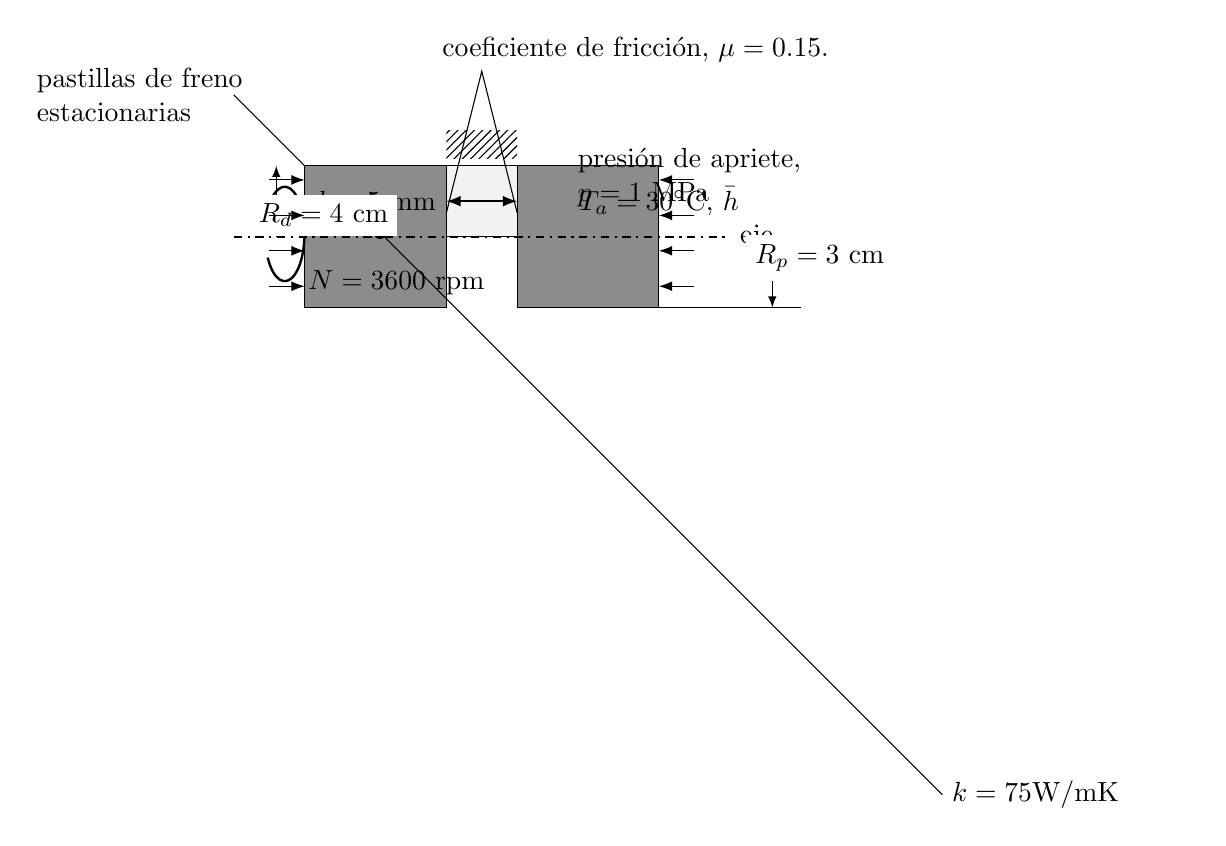
\begin{tikzpicture}[scale=0.9]
\draw[fill=black!5](0,0)rectangle++(\x1,-\y1);
\draw[fill=black!45](0,0)rectangle++(-\x2,-\y2);
\draw[fill=black!45](\x1,0)rectangle++(\x2,-\y2);
\draw[thick,dashdotted](-3*\x1,-\y1)--++(4*\x1,0)node [midway] {\AxisRotator[rotate=0,solid]$N=3600$ rpm}--++(3*\x1,0)node[right]{eje};
\fill[pattern=north east lines,pattern color=black](0,\y2/20)rectangle(\x1,\y2/4);
\draw(0,-\y2/3)--++(\x1/2,\y2)node[pos=1,above, text width=5cm,xshift=2cm]{coeficiente de fricción, $\mu=0.15$.}--++(\x1/2,-\y2);

\draw(-\x2,0)--++(-\x1,\y2/2)node[pos=1, text width=3cm,xshift=-1cm]{pastillas de freno estacionarias};
\draw[thick,latex-latex](0,-\y1/2)--++(\x1,0)node[pos=0,left]{$b = 5$ mm};
\node[]at(3*\x1,-\y1/2){$T_a=30^\circ$C, $\bar h$};

\draw[*-](\x1-\x2,-\y1*7/8)--++(4*\x2,-4*\x2)node[pos=1, text width=3cm,right]{$k=75$W/mK};

\draw[latex-] (\x1,-\y2) --++(2*\x2,0)++(-0.2*\x2,0)--++(0,-\y1+\y2)node[pos=0.7,fill=white,xshift=.6cm]{$R_p=3$ cm}  ;


\draw[latex-] (0,0) --++(-2.*\x1,0)++(-0.2*\x2,0)--++(0,-\y1)node[pos=0.7,fill=white,xshift=.6cm]{$R_d=4$ cm}  ;

\foreach \s in {0.1,...,0.2,0.35,...,.9 }
{\draw[-Latex](-\x1/2-\x2,-\s*\y2)--++(\x1/2,0);
\draw[Latex-](\x1+\x2,-\s*\y2)--++(\x1/2,0);

}
\node[text width=3.5cm] at(3.8*\x1,-\y1/6){presión de apriete, $p = 1$ MPa};
	\end{tikzpicture}
	\end{small}
\end{document}